\documentclass[a4paper]{article}
\usepackage[spanish]{babel}
\usepackage[utf8]{inputenc}
\usepackage{charter}   % tipografia
\usepackage{graphicx}
%\usepackage{makeidx}
\usepackage{paralist} %itemize inline

%\usepackage{float}
%\usepackage{amsmath, amsthm, amssymb}
%\usepackage{amsfonts}
%\usepackage{sectsty}
%\usepackage{charter}
%\usepackage{wrapfig}
\usepackage{listings}
%esto es para formateo del codigo C++
\lstset{
	belowcaptionskip=1\baselineskip,
	basicstyle=\footnotesize,        % the size of the fonts that are used for the code
  	breaklines=true,                 % sets automatic line breaking
  	captionpos=b,                    % sets the caption-position to bottom
  	extendedchars=true,              % lets you use non-ASCII characters; for 8-bits encodings only, does not work with UTF-8
  	keepspaces=true,                 % keeps spaces in text, useful for keeping indentation of code (possibly needs columns=flexible)
  	columns=flexible
  }

\usepackage{color} % para snipets de codigo coloreados
\usepackage{fancybox}  % para el sbox de los snipets de codigo

\definecolor{litegrey}{gray}{0.94}

% \newenvironment{sidebar}{%
% 	\begin{Sbox}\begin{minipage}{.85\textwidth}}%
% 	{\end{minipage}\end{Sbox}%
% 		\begin{center}\setlength{\fboxsep}{6pt}%
% 		\shadowbox{\TheSbox}\end{center}}
% \newenvironment{warning}{%
% 	\begin{Sbox}\begin{minipage}{.85\textwidth}\sffamily\lite\small\RaggedRight}%
% 	{\end{minipage}\end{Sbox}%
% 		\begin{center}\setlength{\fboxsep}{6pt}%
% 		\colorbox{litegrey}{\TheSbox}\end{center}}

\newenvironment{codesnippet}{%
	\begin{Sbox}\begin{minipage}{\textwidth}\sffamily\small}%
	{\end{minipage}\end{Sbox}%
		\begin{center}%
		\vspace{-0.4cm}\colorbox{litegrey}{\TheSbox}\end{center}\vspace{0.3cm}}



\usepackage{fancyhdr}
\pagestyle{fancy}

%\renewcommand{\chaptermark}[1]{\markboth{#1}{}}
\renewcommand{\sectionmark}[1]{\markright{\thesection\ - #1}}

\fancyhf{}

\fancyhead[LO]{Sección \rightmark} % \thesection\ 
\fancyfoot[LO]{\small{Nombre Apellido, Nombre Apellido, Nombre Apellido}}
\fancyfoot[RO]{\thepage}
\renewcommand{\headrulewidth}{0.5pt}
\renewcommand{\footrulewidth}{0.5pt}
\setlength{\hoffset}{-0.8in}
\setlength{\textwidth}{16cm}
%\setlength{\hoffset}{-1.1cm}
%\setlength{\textwidth}{16cm}
\setlength{\headsep}{0.5cm}
\setlength{\textheight}{25cm}
\setlength{\voffset}{-0.7in}
\setlength{\headwidth}{\textwidth}
\setlength{\headheight}{13.1pt}

\renewcommand{\baselinestretch}{1.1}  % line spacing


% \setcounter{secnumdepth}{2}
\usepackage{underscore}
\usepackage{caratula}
\usepackage{url}


%-------------------para algoritmos
\usepackage[]{algorithm2e}
\usepackage[]{algorithmic}
%-------------------------------------------------
\usepackage{amsmath}


% ******************************************************** %
%              TEMPLATE DE INFORME ORGA2 v0.1              %
% ******************************************************** %
% ******************************************************** %
%                                                          %
% ALGUNOS PAQUETES REQUERIDOS (EN UBUNTU):                 %
% ========================================
%                                                          %
% texlive-latex-base                                       %
% texlive-latex-recommended                                %
% texlive-fonts-recommended                                %
% texlive-latex-extra?                                     %
% texlive-lang-spanish (en ubuntu 13.10)                   %
% ******************************************************** %



\begin{document}


\thispagestyle{empty}
\materia{Algoritmos 3}
\submateria{Segundo Cuatrimestre de 2014}
\titulo{Trabajo Práctico II}
\subtitulo{subtitulo del trabajo}
\integrante{Ricardo Colombo}{156/08}{ricardogcolombo@gmail.com.com}
\integrante{Federico Suarez}{610/11}{elgeniofederico@gmail.com}
\integrante{Juan Carlos  Giudici}{827/06}{elchudi@gmail.com}
\integrante{Franco Negri}{893/13}{franconegri2004@gmail.com}
\maketitle
\newpage

\thispagestyle{empty}
\vfill

\thispagestyle{empty}
\vspace{3cm}
\tableofcontents
\newpage

%\normalsize

\section{Plan de vuelo}
\subsection{Introducci\'on} 
Cada participante de una competencia debe cruzar un puente dando saltos de tabl\'on en tabl\'on, teniendo en cuenta que pueden saltar una cantidad m\'axima de tablones de una sola vez. Sin embargo algunos de estos tablones est\'an rotos y se sabe de antemano cuales son los mismos. 
Se desea calcular la cantidad m\'inima de saltos requerida para cruzar el puente.

\subsection{Ejemplos y Soluciones}


\subsection{Desarrollo}
Para la soluci\'on de este problema recurrimos a la tecnica denominada programaci\'on dinamica. 
Por el enunciado sabemos que tenemos n tablones, el participante puede saltar C tablones de una sola vez y cuales son las posiciones de los tablones rotos.Nos armamos dos arreglos donde cada posici\'on representa un tabl\'on, en el primero guardamos 0 y 1 para indicar su estado (sano o roto respectivamente) llenando el mismo seg\'un la entrada, llamemoslo puente, en el otro iremos guardando la cantidad m\'inima de saltos para llegar a cada tabl\'on,llamemoslo Distancias.
Nuestro algoritmo ira recorriendo un tabl\'on por vez, viendo si el mismo esta roto o no. En el caso de que el tabl\'on est\'a roto (seg\'un indica nuestro arreglo puente) continuo al siguiente tabl\'on.
Para los primeros C tablones que estan sanos pondremos 1 en el arreglo Distancias, cuando el algoritmo se encuentre en el tabl\'on i , con C $\leq$ i $\leq $ n-1, calculamos su cantidad m\'inima de saltos de la siguiente manera:\\
- Buscamos el minimo entre i - C y i-1, en el arreglo de Distancias.\\
- Al m\'inimo encontrado le sumamos uno y lo colocamos en la posici\'on i del arreglo Distancias.\\
Una vez completado el arreglo distancias debemos armar el recorrido, para el cual en primer paso buscamos dentro de las C ultimas posiciones del arreglo Distancias el m\'inimo, llamemos j a su posici\'on. Luego agregamos este j a la soluci\'on como el ultimo tabl\'on.
A partir de ah\'i en cada paso buscamos el m\'inimo entre j-C y j-1, y lo agregamos adelante de nuestra soluci\'on y reemplazamos el j con la posici\'on del nuevo m\'inimo. Una vez recorrido todo el arreglo tendremos nuestra soluci\'on optima.
\subsection{Demostraci\'on}

Demostraremos por inducci\'on que en cada paso de este algoritmo obtenemos la m\'inima cantidad de saltos posible para llegar a ese tabl\'on:

Sea P(i) = `` El valor guardado en la posici\'on i-1 del arreglo Distancias es la cantidad m\'inima de saltos hasta el tabl\'on i''

Caso base, P(i) con 0 $\leq$ i $<$ C :
El caso base son los primeros C tablones, donde C es la cantidad m\'axima de tablones que un participante puede saltar de una sola vez. En este caso la cantidad m\'inima de saltos para cada tabl\'on es trivialmente 1, ya que es el primer salto desde el punto de partida.

Paso inductivo, P(n) $ \Rightarrow $ P(n+1) con n $\geq$ C :
Por hip\'otesis inductiva sabemos que tenemos la cantidad de saltos m\'inima hasta el tabl\'on n en el arreglo Distancias (entre las posiciones 0 y n-1). Si el tabl\'on esta roto entonces la cantidad de saltos m\'inima ser\'a infinito. En el caso contrario, para calcular la m\'inima cantidad de saltos para llegar al tabl\'on n+1 revisamos los \'ultimos C tablones previos, y nos quedamos con el que requiera la menor cantidad de saltos para llegar hasta el, y llamaremos a esta cantidad Min. Entonces la cantidad m\'inima de saltos para llegar al tabl\'on n+1 seria Min+1, y ahora veremos que efectivamente lo es.
Si Min+1 no fuera la cantidad m\'inima de saltos para llegar al tabl\'on n+1 entonces existe un tabl\'on entre n-C y n-1 cuya cantidad m\'inima de saltos para llegar hasta el es menor a Min, lo cual es absurdo porque seleccione al m\'inimo.
Puede pasar que exista un tabl\'on entre n-C y n-1, distinto al seleccionado, cuya cantidad m\'inima de saltos para llegar hasta el coincida con Min. En ese caso esta soluci\'on es tan buena como la m\'ia. Por lo tanto la cantidad de saltos m\'inima para llegar al tabl\'on n+1 es efectivamente Min+1.

Para armar el recorrido, realizamos lo ya descripto en la secci\'on de desarrollo y como siempre vamos tomando el m\'inimo en cada paso recorriendo el arreglo Distancias hacia atr\'as llegamos a una soluci\'on optima, que como vimos previamente, puede haber mas de una. 



\subsection{Complejidad}
El siguiente es un pseudo-c\'odigo de nuestro algoritmo.\\
\begin{algorithm}
\begin{algorithmic}[1]\parskip=1mm
 \caption{ \\Saltos( saltoMax : natural, puente : arreglo(1's y 0's), distancias: arreglo(naturales) , cantidadTablones : natural)}
		\STATE{Si saltoMax > cantidadTablones} \;\;\tOde{1}
		\STATE{\quad devolver 1} \;\;\tOde{1}
		\STATE{posActual \leftarrow 0}  \;\;\tOde{1} \\
		\STATE{SI NO}\\
		\STATE{mientras posActual < cantidadTablones} \;\; \tOde{1}
			\STATE{\quad SI puente.indice(posActual) es 0} \;\; \tOde{1}
				\STATE{\quad\quad posActual \leftarrow posActual + 1} \;\; \tOde{1}\\
			\STATE{\quad SI NO}
				\STATE{\quad\quad SI posActual - saltoMax < 0} \;\;\tOde{1}
					\STATE{\quad\quad\quad distancias.indice(posActual) \leftarrow 1}\;\; \tOde{1}\\
					\STATE{\quad\quad\quad posActual \leftarrow posActual + 1} \;\;\tOde{1}\\
				\STATE{\quad\quad SI NO}
					\STATE{\quad\quad\quad minimoSalto \leftarrow BUSCOMINIMO(posActual  - saltoMax, posActual, puente)} \;\; \tOde{saltoMax} \\
					\STATE{\quad\quad\quad distancias.indice(posActual) \leftarrow minimoSalto + 1}\;\; \tOde{1}\\
					\STATE{\quad\quad\quad posActual \leftarrow posActual + 1} \;\;\tOde{1}\\
\\
Todas las asignaciones y comparaciones son en \Ode{1} como esta marcado en el pseudocodigo, para el caso de la funci\'on BuscoMinimo, esta recorre en el arreglo puente buscando el m\'nimo entre las posiciones posActual-saltoMax y posActual, esto tiene una complejidad del orden \Ode{saltoMax}. \\
El ciclo de las lineas 4 - 14 se realiza n veces con lo cual la complejidad total del algoritmo es \Ode{n*saltoMax}, como saltoMax es una constante menor a n la complejidad total del algoritmo es \Ode{n}.
\end{algorithmic}
\end{algorithm}			
			
			
\subsection{Experimentacion}

  

 


\clearpage

\section{Caballos salvajes} 
\subsection{Introduccion} 
Se esta diseñando un software de arquitectura, para el cual es necesario que dado un conjunto de edificios representados como rectangulos apoyados sobre una base en comun, se devuelva el perfil definido en el horizonte.\\
Estos edificios vienen representados por tuplas de tres elementos que representan donde comienza el edificio, su altura y donde termina, de las cuales tenemos que ir tomando en cada momento donde comienza un edificio la altura maxima alcanzada en ese punto.

 \subsection{Ejemplos y Soluciones}
 Consideremos el siguiente ejemplo del problema:\\
 $ [<3,2,5>;<1,4,2>;<4,1,6>;<6,8,10>]$ \\
  Cada una de estas tuplas de tres elementos se indica donde comienza el edificio en la primera coordenada, su altura en la segunda y donde termina en la tercera coordenada.\\
  
  Lo primero que hacemos es ordenar estas tuplas en orden creciente por lo que representa donde comienza el edificio (llamemosla pared izquierda), quedandonos de la siguiente manera:\\ 
$[<1,4,2>;<3,2,5>;<4,1,6>;<6,8,10>$] \\

Por otro lado ordenamos los edificios por la coordenada donde terminan (llamemosla pared derecha).\\
$[<1,4,2>;<3,2,5>;<4,1,6>;<6,8,10>$] \\

\subsection{Desarrollo}
Como mencionamos anteriormente, tenemos como datos de entrada la posici\'on donde comienza y termina cada edificio y adem\'as su altura, con lo cual representaremos a los edificios con tuplas de 3 elementos (posici\'on de inicio o pared izquierda, altura, y posici\'on donde termina o pared derecha). Primero organizaremos a los edificios en dos arreglos, donde cada arreglo contendr\'a el total de edificios, uno con un orden ascendente seg\'un pared izquierda y el otro tambi\'en con un orden ascendente pero seg\'un pared derecha. Adem\'as tendremos un conjunto en el que iremos agregando los edificios que ``comience'' y quitando los edificios que ``terminen'', es decir, aqu\'i� estar\'an los edificios ``activos'' (que ``empezaron'' y no ``terminaron'') en cada momento.
La idea del algoritmo es ir recorriendo las posiciones (del eje x) en las que haya una o m\'as paredes. En cada punto lo que haremos es agregar a mi conjunto de activos los edificios que en ese punto tengan su pared izquierda, o sea que est\'an "comenzando", y quitar a los edificios que all\'i tengan su pared derecha, o sea que est\'an ``terminando''. Una vez completada esta labor, buscaremos el edificio activo que tenga la altura m\'axima y nos lo guardaremos, llam\'emoslo Max. Se puede ver claramente que el borde superior de la silueta en un punto dado va a estar determinado por el edificio m\'as alto que haya en ese punto, es decir, el edificio activo m\'as alto. Como en cada paso podemos conseguir el edificio activo m\'as alto, proseguiremos as\'i� hasta el \'ultimo punto y habremos arm\'andonos la silueta.

\subsection{Demostraci\'on}
Demostraremos por inducci�n que en cada paso de este algoritmo obtenemos la altura del edificio m�s alto en ese punto.

P(i) = "Nuestro conjunto de edificios activos contiene todos los edificios que empezaron entre el punto de inicio y el punto i inclusive y que a�n no han terminado, es decir, terminan en un punto estrictamente mayor que i"

Caso base, P(1):
En este caso nos encontramos con nuestro primer conjunto de paredes, que puede tener una o m�s paredes. Este s�lo puede tener paredes izquierda ya que es donde comienzan nuestros primeros edificios y ning�n edificio ha empezado antes como para que aparezca una pared derecha indicando su finalizaci�n. Por lo tanto s�lo tenemos un conjunto de edificios que comienzan en este punto, los cuales agregaremos a nuestro conjunto de edificios activos. Es claro ver que el conjunto de edificios activos ahora tiene todos los edificios que comenzaron y no han terminado hasta el primer punto inclusive ya que ning�n edificio termina aqu� como previamente hemos dicho y entonces todos estos empezaron y no terminaron.

Paso inductivo, P(n) $\rightarrow$ P(n+1):
Nuestra hip�tesis inductiva nos dice que nuestro conjunto de edificios activos contiene todos los edificios que empezaron entre el punto de inicio y el punto n inclusive, y que a�n no han terminado. Ahora veamos qu� ocurre en n+1. En este punto podemos encontrar un conjunto que contiene tanto paredes izquierda como derecha, con lo cual separaremos a este conjunto de paredes en dos subconjuntos. Por un lado el conjunto de paredes izquierda, llam�mosle I, y por otro el de paredes derecha, llam�mosle D. Recorreremos primero el conjunto I agregando cada edificio de este conjunto al conjunto de edificios activos, es decir, agregaremos todos los edificios que comienzan en este punto.
Acto seguido, recorreremos el conjunto D quitando cada edificio que aparezca en este conjunto de nuestro conjunto de edificios activos ya que todos estos edificios est�n terminando y por lo tanto ya no deben pertenecer a nuestro conjunto. Veamos ahora que efectivamente se est� cumpliendo P(n+1). Los edificios agregados en este paso no pueden terminar aqu� mismo, ya que eso implicar�a que est�n empezando y terminando en la misma posici�n, lo cual no es v�lido. Por lo tanto estar�an terminando en un punto estrictamente mayor a n+1. 
Los edificios que terminaban en el paso n+1 fueron ya removidos del conjunto. Ahora miremos qu� pasa con los dem�s edificios que ya estaban en nuestro conjunto de edificios activos y no fueron eliminados. Por hip�tesis inductiva, estos edificios no tienen su pared derecha entre el punto de inicio y el punto n, es decir, terminan en un punto estrictamente mayor que n. Pero como no fueron borrados de nuestro conjunto, quiere decir que no tienen su pared derecha en n+1, o sea que terminan en un punto estrictamente mayor a n+1. Entonces vale P(n+1).


Teniendo nuestro conjunto de edificios activos, en cada punto podemos buscar el edificio de mayor altura y registrar los cambios de altura cada vez que empieza y/o termina un edificio. Luego, es trivial armarnos la silueta ya que, con las fluctuaciones de las alturas m�ximas a lo largo de nuestra ciudad, ya tenemos su borde superior en cada tramo.


\subsection{Complejidad}

definimos edificio = < izq :natural x alto : natural x der : natural >
definimos edificioenCero al que tiene todos sus elementos en cero.
\begin{algorithm}
\begin{algorithmic}[1]\parskip=1mm
 \caption{LaSilueta( ciudad: arreglo(edificios) , cantidadEdificios : natural)}
	
	\STATE{arregloXIzq \leftarrow ordenarXIzquierda(ciudad)}\\
	\STATE{arregloXDer \leftarrow ordenarXDerecha(ciudad)}\\
	\STATE{EdificiosActivos \leftarrow Multiconjunto(edificio)}\\
	\\
	\STATE{posIzquierdo , posDerecho \leftarrow 0}\\
	\STATE{max \leftarrow edificioenCero \\
	\STATE{mientras posIzquierdo < cantidadEdificios \&\& posDerecho < cantidadEdificios }\\
	\STATE{ \quad SI arregloXIzq.indice(posIquierdo).izq \leq arregloXDer.indice(posDerecho).der}\\
			\STATE{\quad\quad auxiliar \leftarrow arregloXIzq.indice(posIzquierdo)}\\
			\STATE{\quad\quad mientras auxiliar.izq = arregloXIzq.indice(posIquierdo).izq \&\& posIzquierdo != cantidadEdificios}\\
			\STATE{\quad\quad\quad agregar(arregloXIzq.indice(posIquierdo), EdificiosActivos )}\\
			\STATE{\quad\quad\quad SI arregloXIzq.indice(posIquierdo).alto > max.alto}\\
			\STATE{\quad\quad\quad\quad max \leftarrow arregloXIzq.indice(posIquierdo) }\\
		\STATE{\quad SI NO }\\
			\STATE{\quad\quad auxiliar \leftarrow arregloXDer.indice(posDerecha)}\\
			\STATE{\quad\quad mientras auxiliar.der = arregloXDer.indice(posDerecha).der && posDerecha != cantidadEdificios}\\
			\STATE{\quad\quad\quad SI  arregloXDer.indice(posDerecha).id = max.id}\\
			\STATE{\quad\quad\quad\quad dameMaximoSiguiente( arregloXDer.indice(posDerecha), EdificiosActivos)}\\
			\STATE{{\quad\quad\quad\quad sacar( arregloXDer.indice(posDerecha), EdificiosActivos)}
\\
\end{algorithmic}
Los algoritmos ordenarXizquierda y ordenarXDerecha es el conocido algoritmo mergeSort sacado del libro de brassard, la complejidad del mismo es \Ode{N*Log(N)} siendo N la cantidad de elementos en el arreglo, �sea todos los edificios, estos algoritmos ordenan los arreglos de tuplas, uno por la coordenada izq y el otro por la coordenada derecha respectivamente.\\
El multiconjunto EdificiosActivos esta representado con la estructura Multiset de la librer�a STL de c++, la relaci\'on de orden sobre los elementos que se defini\'o es por la coordenada alt y en el caso que la altura sea igual por la componente der.\\
Para las operaciones para agregar, sacar elementos la complejidad es \Ode{log(n)} siendo n la cantidad de elementos en el multiconjunto y para obtener el proximo maximo lo que se realiza es obtener la referencia al elemento que 
representa el m\'aximo, esto lleva \Ode{Log(n)} y luego se obtiene el posterior, en caso de no ser posible obtenemos el anterior, en el peor caso se tienen todos los edificios y la complejidad seria \Ode{log(N)}.\\
El ciclo de las lineas 9-12 se realiza para cada punto x donde haya paredes izquierdas, con lo cual la complejidad total sera la suma de todas las paredes izquierda, siendo esta N la cantidad de edificios. De la misma manera el ciclo de las lineas 15 a 18 se ejecuta para todas las paredes derechas de los edificios con lo cual el total de las iteraciones sera la suma de las paredes derechas �sea N. Como el ciclo principal se ejecuta mientras la cantidad de paredes recorridas izquierdas sea menor a la cantidad de edificios y la cantidad de paredes derechas sea menor a la cantidad de edificios y las iteraciones internas modifican las paredes izquierdas y derechas recorridas, el total de las iteraciones es 2*N, siendo N la cantidad total de edificios, con lo cual como la complejidad de agregar , sacar y obtener el m\'aximo es \Ode{log(N)} en el peor caso, el total es \Ode{2*N*Log(N)} $\subset$ \Ode{N*Log(N)} siendo esta la complejidad total del algoritmo y esta estrictamente menor a \Ode{N^2} como se solicitaba en el enunciado.

\end{algorithm}	
\newpage
\subsection{Experimentaci\'on}
Se realizaron experimentaciones sobre varios tipos de caso para observar el comportamiento del algoritmo, en todos los casos se generaron 1000 entradas, a las gr�ficas resultantes se las comparo con la funci�n n*log(n)*1000, siendo n la cantidad de edificios de entrada.\\
Para la primer ejecuci�n se realizo un an\'alisis sobre el algoritmo en edificios donde la distancia entre sus paredes izquierda y derecha era corta, estas se encontraban entre las posiciones 1 y 30, pero sus alturas variaban en el orden entre 1 y 10000, dando el siguiente gr�fico como resultado.\\

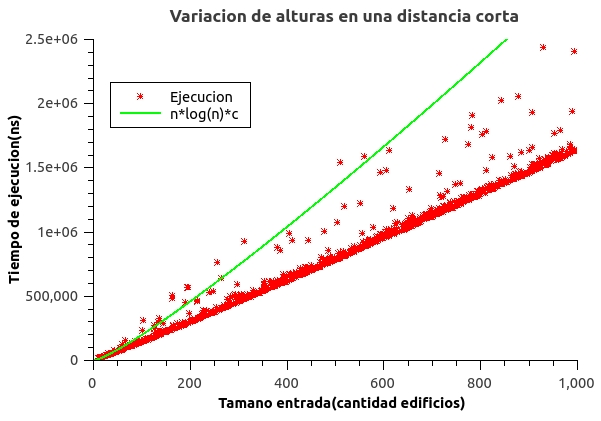
\includegraphics[scale=0.7]{Ej2/VariacionAlturas.jpg}\\

El segundo gr\'afico corresponde a instancias generadas de manera random donde la altura se encontraba entre 1 y 40, pero las distancias entre la primer y la segunda pared de cada edificio varia entre los 1 y 2000 , elegido de manera random la posici�n de ambos lados pero siempre que sea entrada valida, \'osea el valor de la pared izquierda es mayor estricta a la de la pared derecha.

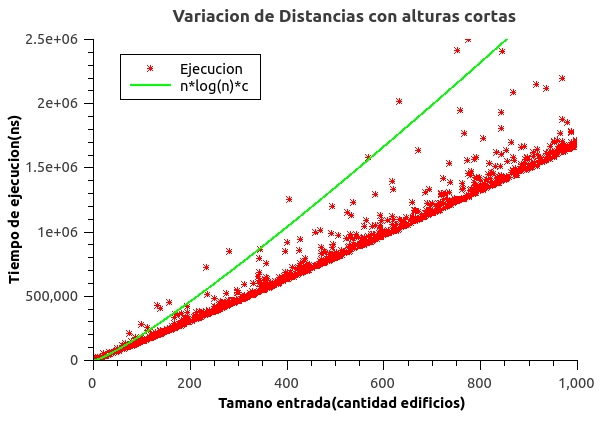
\includegraphics[scale=0.7]{Ej2/VariacionDistancias.jpg}


Luego para el tercer gr\'afico consideramos que era importante ver como se comportaba el multiconjunto cuando se agregaban todos los edificios de la entrada, de esta manera se generaron entradas donde los edificios eran todos iguales, as\'i se ingresaban todos al multiconjunto y ve\'iamos como se comportaba el algoritmo, obteniendo este gr\'afico como resultado donde se ve que su complejidad es del orden logar\'itmico en la cantidad de edificios de entrada por la cantidad edificios.

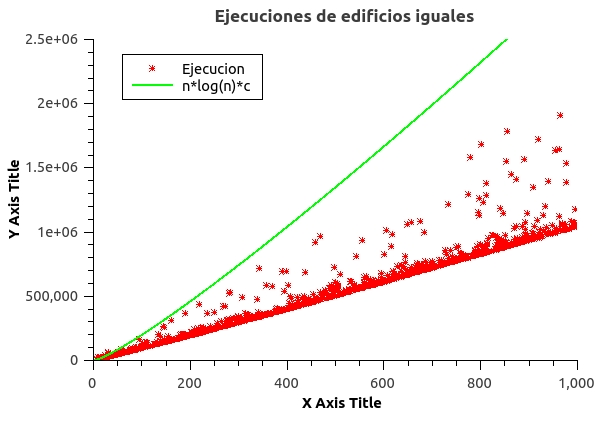
\includegraphics[scale=0.7]{Ej2/iguales.jpg}\\
Por ultimo realizamos un gr�fico con entradas random donde las mismas variaban combinando todas las anteriores, obteniendo de nuevo que el orden era logar�tmico al compararlo con la funci�n.

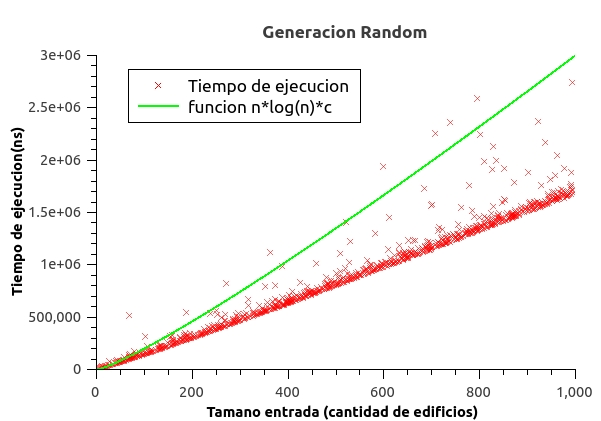
\includegraphics[scale=0.7]{Ej2/Random.jpg}\\

 Concluimos por lo tanto que el algoritmo respeta los ordenes de complejidad requeridos.





\clearpage

\section{La comunidad del anillo}
\section{Introducci\'on}
El problema para este ejercicio es el siguiente, se nos presentan $n$ productos qu\'imicos, los cuales deben transportarse en camiones de un lugar a otro, el llevar al elemento $i$ en el mismo cami\'on que otro elemento $j$, conlleva una ''peligrosidad'' asociada $h_i_j$. El objetivo del algoritmo ser\'a encontrar la soluci\'on que utilize la menor cantidad de cami\'ones posibles, pero que cada cami\'on tenga una peligrosidad menor a una cota $m$.
\\
La entrada del problema consiste en:
\\
\begin{itemize}
\item Un entero \textbf{n} $\rightarrow$ Representar\'an el n\'umero de productos qu\'imicos a transportar.
\item Un entero \textbf{m} $\rightarrow$ Representar\'a la cota de peligrosidad que ningun cami\'on puede superar.
\item \textbf{n-1} filas donde, para cada fila $i$ consta de $n-i$ enteros:
\begin{itemize}
\item $h_i_{,i+1}, h_i_{,i+2}$ ... $h_i_{,n}$ $\rightarrow$ Representar\'an la peligrosidad asociada del elemento $i$ con los elementos $i+1$, $i+2$ ... $n$.
\end{itemize}
\end{itemize}
\\
La salida, por su parte, constar\'a de una fila con:
\\
\begin{itemize}
\item Un entero \textbf{C} $\rightarrow$ Representar\'a la cantidad indispensable de cami\'ones que es necesaria para transportar los productos bajo las condiciones del problema.
\item $n$ enteros $\rightarrow$ Representar\'an en que cami\'on viaja cada producto.
\end{itemize}

\subsection{Ejemplo de entrada valida}
Hagamos un peque�o ejemplo para que pueda ilustrarse bien el problema.
\\
Supongamos que tenemos $3$ productos qu\'imicos, el producto $1$ es muy inestable, por lo que si es transportado con el producto $2$ la peligrosidad asociada al camion en el que viajan estos dos productos asciende a $40$, y si se transporta con el producto $3$ la peligrosidad ser\'a de $35$. El producto $2$ en cambio es de naturaleza mas estable, por lo que si es transportado con el producto $3$ solo produce una peligrosidad de $3$.
\\
Por otro lado queremos que la peligrosidad por cami\'on no supere el valor de $39$.
\\
Entonces la entrada para este problema ser\'a:
\\
\\
$\textbf{3 39}$
\\
$\textbf{40 35}$
\\
$\textbf{3}$
\\
\\
Para una entrada de estas dimenciones es posible buscar la mejor solucio\'on a mano.
\\
Las posibles combinaciones son que los tres productos viajen juntos, que los tres viajen separados en camiones distintos, que $1$ y $2$ viajen juntos en el mismo camion y el producto $3$ viaje en otro cami\'on diferente, que $1$ y $3$ viajen juntos y el $2$ separado y que $2$ y $3$ viajen juntos y el producto sobrante viaje en otro cami\'on.
\\
La primera d\'a una peligrosidad de $40+35+3$ por lo la cota de peligrosidad se ve superada, lo que lo vuelve una soluci\'on inviable, la segunda es valida, ya que la peligrosidad de cada camion es $0$, pero se necesitan $3$ camiones. Que $1$ y $2$ viajen juntos, tampoco es valida, la peligrosidad de ese camion es demaciado alta, y finalmente las ultimas dos son validas (peligrosidad $35$ y $3$, respectivamente) y solo son necesarios dos camiones.
\\
Es claro, luego, que las dos ultimas soluciones son las que el algoritmo podr\'ia devolever.
\\
Luego las dos salidas que podr\'a devolver el algoritmo son:
\begin{itemize}
\item $2$ $1$ $2$ $1$
\end{itemize}
o
\begin{itemize}
\item $2$ $1$ $2$ $2$
\end{itemize}
\\
\section{Idea General de Resoluci\'on}
Luego la idea del algoritmo es simple, probar todas las combinaciones posibles de camiones y de entre todas determinar cual es la que cumple con la cota de peligrosidad pedida y usa la menor cantidad de camiones posible. Ademas, para aumentar la performance del algoritmo, se ir\'an podando ramas de la familia de soluciones de manera tal de que no sea necesario chequear absolutamente todos los casos.
\\
Antes de presentar el pseudocodigo vale aclarar un punto importante y es que el algoritmo debe encontar siempre una soluci\'on. Esto se debe a que siempre es posible poner todos los productos qu\'imicos en camiones separados, lo que nos d\'a  una peligrosidad $0$. Es posible usar esta como una cota contra la cual parar de chequear, si tenemos $n$ productos qu\'imicos, es simple ver que a lo sumo usar\'emos $n$ camiones. Denominaremos a esta como la "peor soluci\'on" ya que es claro que es una soluci\'on valida, pero que usa la maxima cantidad de camiones.
\\
En cuanto a las podas, utilizamos dos, una que en cada paso del backtrack chequea si la soluci\'on final que encontramos hasta el momento usa una cantidad menor de camiones que la solucion parcial que se esta construyendo. Es claro que de ser as\'i, estamos la solucion parcial nunca podr\'a ser mejor, por lo tanto se podar\'a toda esa familia de soluciones.
\\
La segunda chequea que la soluci\'on parcial que estamos construyendo no exceda el limite de peligrosidad pedido por el ejercicio, en caso de ser as\'i la soluci\'on no ser\'a valida. En caso de que esto suceda, tambien se poda.
\\
Finalmente el pseudocodigo para resolver este problema queda as\'i:

\begin{algorithm}
\begin{algorithmic}[1]\parskip=1mm
\caption{void FuncionPrincipal()}

  \STATE{Generar una matriz con las peligrosidades entre los distintos productos}
  
  \STATE{Se inicializa la solucion final, como la peor de las soluciones}
  
  \STATE{Backtrack(tablaDePeligrosidad, solucionParcial, solucionFinal)}
  
  \STATE{Mostar la soluci\'on final}
 
 \end{algorithmic}
\end{algorithm}

\begin{algorithm}
\begin{algorithmic}[1]\parskip=1mm
\caption{Bool Backtrack(tablaDePeligrosidad, solucionParcial, solucioninal)}
	
	\STATE{Llamo a la funcion check(tablaDePeligrosidad, solucionParcial, solucionFinal)}
	
	\STATE{\quad Si check devuelve $2$, la solucion parcial es mejor que la final}
	\STATE{\quad \quad Pongo la solucion parcial como final} 
	\STATE{\quad \quad Corto la recursi\'on y busco por otra rama}

	\STATE{\quad Si check devuelve $0$, la cota de peligrosidad fu\'e sobrepasada}
	\STATE{\quad \quad esta rama no me sirve, podo}	

	\STATE{\quad Si check devuelve $3$, la solucion anterior usa menos camiones}
	\STATE{\quad \quad esta rama no me sirve, podo}

	\STATE{\quad Si check devuelve $1$, la solucion es valida, pero no est\'a completa}
	\STATE{\quad \quad contin\'uo agregando camiones}

	\STATE{Para cada valor $i$ de $1$ hasta $n$ prueba meter el siguiente producto de la lista en el camion $i$ y se llama a la funcion Backtrack()}
\end{algorithmic}
\end{algorithm}

\begin{algorithm}
\begin{algorithmic}[1]\parskip=1mm
\caption{int check(tablaDePeligrosidad, solucionParcial, solucionFinal)}


	\STATE{Checkeo si la solucion final usa menos camiones ~~~~~~~~~~~~ $O(n)$}
	\STATE{\quad Si es verdad}
	\STATE{\quad \quad Devuelvo $3$}


	\STATE{Checkeo si la cota de peligrosidad fue sobrepasada ~~~~~~~~~~~~ $O(n^2)$}
	\STATE{\quad Si es verdad}
	\STATE{\quad \quad Devuelvo $0$}


	\STATE{Checkeo si la cada producto tiene un camion asignado ~~~~~~~~~~~~ $O(1)$}
	\STATE{\quad Si es verdad}
	\STATE{\quad \quad Devuelvo $2$}

\STATE{Devuelvo $1$}

\end{algorithmic}
\end{algorithm}

\newpage
\section{Correctitud}
Seg\'un lo desarrollado en la idea principal, sabemos que el algoritmo siempre tend\'a una soluci\'on y esta se encuentra acotada en un vector de $n$ elementos cada uno entre $1$ y $n$. Dado que el rango es acotado, un algoritmo que chequee todas las posibles soluciones y devuelva la soluci\'on valida que usa menos camiones, ser\'a un algoritmo correcto.
\\
Ahora lo que resta demostrar es que las podas que realizamos, no quitan soluciones v\'alidas.
\\
La primera de las podas chequea que si la soluci\'on parcial excede la cota $m$. Es claro ver que cualquier soluci\'on que tenga una sub-soluci\'on inv\'alida nunca podr\'a ser v\'alida, por lo tanto se puede descartar sin necesidad de completarla.
\\
La segunda de las podas chequea que la soluci\'on que estamos construyendo tenga menos camiones que la mejor soluci\'on que tenemos hasta el momento. Esto es, si s\'e que puedo llevar los $n$ productos qu\'imicos en $j$ camiones, no es necesario explorar las soluciones que contengan m\'as de $j$ camiones, estas soluciones jam\'as podr\'an ser mejores que la soluci\'on que ya tengo.
\\
Luego quitando esa parte del espacio de soluci\'ones no estoy quitando en ningun momento posibles soluciones \'optimas, ergo, el algoritmo es correcto.  
\\
\section{Complejidad}
Por cada producto qu\'imico, el algoritmo de backtrack intenta ponerlo en cualquiera de los $n$ posibles camiones, y realiza $O(n^2)$ chequeos intentando podar.
\\
Entonces la formula quedar\'a:
\\
$$T(i) = T(i-1)n + n^2$$
\\
$$T(1) = n + n^2$$
\\
Luego para el peor de los casos el algoritmo tendr\'a una complejidad de $O(n^n)$.
\\
\section{Resultados}
\subsection{Testing}

\subsection{Caso Random}
Para testear la performance de nuestro algoritmo se cre\'o un generador de entradas que fabricar\'a instancias random del problema. Luego se comparar\'a el tiempo que tarda nuestro algoritmo contra uno que encuentre la soluci\'on utilizando fuerza bruta y tambi\'en contra otro backtracking, pero con las podas invertidas, o sea primero chequea si la cantidad de camiones de la soluci\'on parcial es menor a la cantidad de camiones de la mejor soluci\'on hasta el momento y luego chequea que la cota de peligrosidad sea la correcta, para ver si esto var\'ia de alguna manera la complejidad.
\\
El testeo consisti\'o en generar 40 instancias del problema para cada $n$ diferente, con un $m$ fijo y valores de peligrosidad entre productos qu\'imicos que var\'ian entre $1$ y $m$. Luego se tom\'o la media y compararon los resultados:
\\
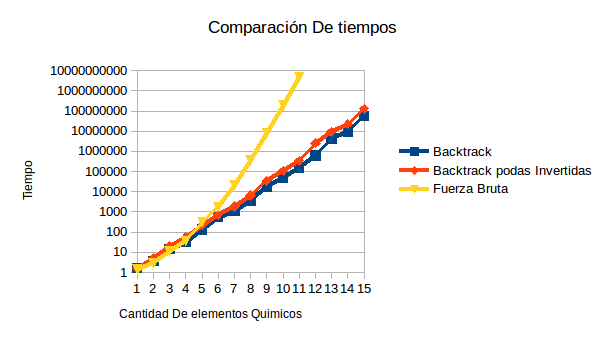
\includegraphics[width=18cm]{./Ej3/graph1.png}
\\
En el gr\'afico puede verse que nuestro algoritmo es notablemente superior a un algoritmo de fuerza bruta, ya que escala mucho mejor con respecto a $n$ y levemente mejor al backtracking con las podas invertidas. Para los casos de $14$ y $15$ elementos el backtracking pudo arrojar una respuesta en un tiempo admisible, mientras que el de fuerza bruta ya tardaba tiempos completamente fuera de escala.
\\
Para comprobar de manera experimental que la complejidad del algoritmo solo depende de $n$ tambi\'en se realiz\'o lo mismo variando la cota de peligrosidad $m$, para un $n$ fijo igual a $9$.
\\
Los resultados arrojados pueden verse en el siguiente gr\'afico:
\\
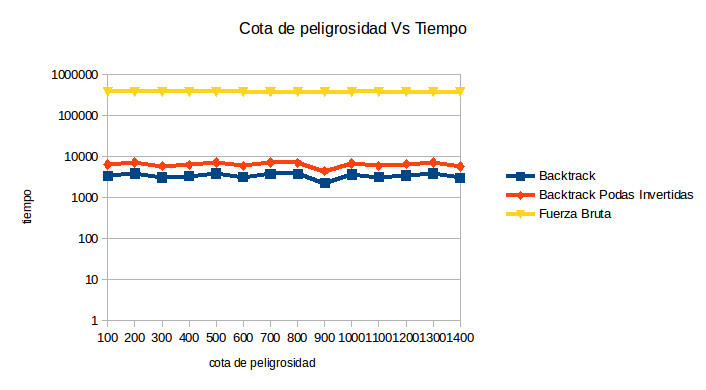
\includegraphics[width=18cm]{./Ej3/graph2.png}
\\
Luego es claro que ninguno de los algoritmos depende de $m$. Adem\'as en este gr\'afico puede volverse a apreciar de manera visible la mejora de nuestro algoritmo con respecto a uno de fuerza bruta.
\\
\subsection{Peor caso}
Otro test que podemos intentar realizar es ver si nuestro algoritmo presenta alguna mejora al de fuerza bruta en el peor de los casos, esto es, en el caso de que cada producto tenga que viajar forzosamente en un cami\'on diferente, obligando de cierta manera a nuestro algoritmo a chequear todos los reslutados posibles, sin poder realizar podas significativas.
\\
Para testear esto tomamos nuevamente $40$ muestras aleatorias, con un $m$ fijo en $10$, valores de peligrosidad los productos entre $m$ y $m+2$ las corremos en los tres algoritmos.
\\
Los resultados pueden verse en el siguiente cuadro:
\\
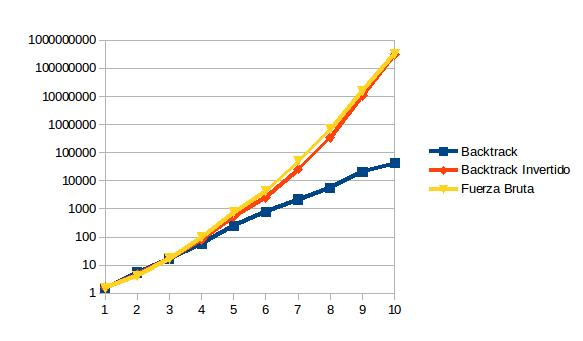
\includegraphics[width=18cm]{./Ej3/peorGraph.jpg}
\\
Puede verse aqu\'i que nuestra soluci\'on contin\'ua siendo mejor que uno de fuerza bruta. En este caso, el otro backtracking con las podas invertidas muestra una notable perdida de performance, siendo casi tan malo como el algoritmo de fuerza bruta.


\section{Adiconales}
1) y 2)Ahora que los camiones no son homogeneos, se ampl\'ia el espacio de soluci\'ones a explorar, ya que, por ejemplo, antes con tres camiones homogeneos, bastaba chequear las soluciones:

\begin{itemize}
\item 1 2 3
\item 1 1 2
\item 1 1 1
\item 1 2 1
\end{itemize}

Ahora que los camiones no son uniformes, esto ya no es as\'i, ya que la cota de peligrosidad por camion var\'ia. Por lo tanto ahora se dever\'an explorar las siguientes soluci\'ones:

\begin{itemize}
\item 1 2 3
\item 1 1 1
\item 2 2 2
\item 3 3 3
\item 1 1 2
\item 1 1 3
\item 2 2 1
\item 2 2 2
\item 3 3 1
\item 3 3 2
\item 1 2 3
...
\end{itemize}

En resumen, pasamos de tener que chequear $4$ posibles combinaciones a $27$.

Dicho para cualquier cantidad $n$ de productos quimicos, ahora tendr\'emos que chequear $n^n$ combinaciones diferentes cuando antes solo ten\'iamos que chequear $\frac{(2n-1)!}{n!(n-1)!}$ posibilidades (Esto se obtiene por combinatoria, es elegir para cada producto un cami\'on $n$, sin que importara el orden y pudiendo repetir).

Luego se ve que el espacio de soluciones se ampl\'ia enormemente, por lo que el tiempo de ejecuci\'on del algoritmo ser\'a mucho peor.

En nuestro caso, ambas podas se podr\'an aplicar al algoritmo, oesa, tanto la poda que chequeaba si la mejor soluc\'on que encontr\'e hasta ahora sigue valiendo utiliza menos camiones que la que estoy construllendo en este momento, como la poda que chequeaba la cota la cota de peligrosidad en cada paso esta siendo sobrepasada, siguen siendo aplicables, con la peque�a modificaci\'on que al chequear esto ultimo se debe tener en cuenta en que cami\'on se estan poniendo los productos quimicos.

\clearpage

\section{Aclaraciones}
\section{Medicion de los tiempos}

Para este tp como trabajamos bajo el lenguaje de programacion C++, decidimos calcular los tiempos utilizando 'chrono' de la libreria standard de c++ (chrono.h) que nos permite calcular el tiempo al principio del algoritmo y al final, y devolver la resta en la unidad de tiempo que deseamos.\\ \\


\section{C\'odigo Fuente}
\subsection{Ej1.cpp}
\lstinputlisting[language=C++]{Ej1/ej1.cpp}

\newpage
\subsection{Ej2.cpp}
\lstinputlisting[language=C++]{Ej2/ej2.cpp}

\newpage
\subsection{Ej3.cpp}
\lstinputlisting[language=C++]{Ej3/ej3.cpp}




\end{document}

